\input{praeambel_gesina.tex}

\usepackage{pgf,tikz}
\usetikzlibrary{arrows}


\begin{document}
\centering


%5.1.2 Das Bisektionsverfahren
	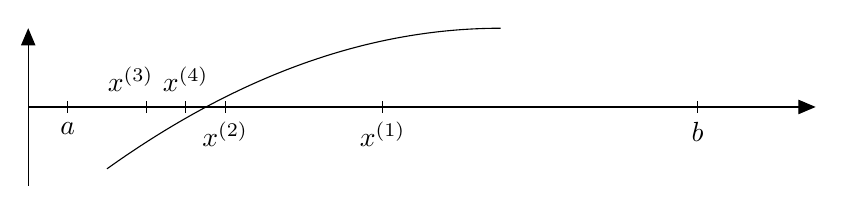
\begin{tikzpicture}[>=triangle 45]
		\draw[->] (0,0) -- (10,0);
		\draw[->] (0,-1) -- (0,1);
		\draw[smooth,samples=100,domain=1:6] plot(\x,{1-1/14*((\x-6)^2)});
		
		\foreach \x/\xtext in
			{0.5/a,4.5/{x^{(1)}},2.5/{x^{(2)}},8.5/b}
				\draw(\x,2pt)--(\x,-2pt) node[below] {$\xtext$};
				
		\draw (1.5,-2pt) -- (1.5,2pt);
		\draw (1.3,2pt) node[above] {$x^{(3)}$};
		\draw (2,-2pt) -- (2,2pt) node[above] {$x^{(4)}$};
	\end{tikzpicture}
	
% 5.2.1a) Beispiel
	\begin{tikzpicture}[>=triangle 45,scale=2]
		\draw[->] (0,0) -- (4.4,0);
		\draw[->] (0,0) -- (0,3);
		\draw[smooth,samples=100,domain=-0.5:3.8] plot(\x,{1+exp(-\x)});
		\draw (3.8,1) node[right] {$g_1(x)$};
		\draw[smooth,samples=100,domain=0:2] plot(\x,{\x});
		\draw[dash pattern=on 3pt off 3pt] (0,1.818730753) node[left] {$x^{(1)}$} -- (0.2,1.818730753) -- (0.2,0) node[below] {$x^{(0)}$};
		\draw[dash pattern=on 3pt off 3pt] (0,1.162231532) node[left] {$x^{(2)}$} -- (1.818730753,1.162231532) -- (1.818730753,0) node[below] {$x^{(1)}$};
		\draw[dash pattern=on 3pt off 3pt] (0,1.312787406) node[left] {$x^{(3)}$} -- (1.162231532,1.312787406) -- (1.162231532,0) node[below] {$x^{(2)}$};
	\end{tikzpicture}
	
%5.2.1b) 
	\begin{tikzpicture}[>=triangle 45,scale=2,x=1.5cm,y=0.7cm]
			\draw[->] (0,0) -- (3,0);
			\draw[->] (0,0) -- (0,3);
			\draw[smooth,samples=100,domain=1.07:2.8] plot(\x,{-ln(\x-1)});
			\draw[smooth,samples=100,domain=0:2] plot(\x,{\x});
			
			\draw(1,2pt) -- (1,-2pt) node[below left] {1};
			\draw(2,2pt) -- (2,-2pt) node[below] {2};
			\draw[dash pattern=on 3pt off 3pt] (1.2,0) node[below] {$x^{(0)}$} -- (1.2,1.609437912);
			\draw[dash pattern=on 3pt off 3pt] (1.609437912,0) node[below] {$x^{(1)}$} -- (1.609437912,1.609437912);
	\end{tikzpicture}
	
	(Notiz: $x^{(2)}$ nicht im Definitionsbereich)
	
%Veranschaulichung einer Kontraktion
	\begin{tikzpicture}
		\draw (0,4) node[below right] {$u$} -- (3,4) node[below left] {$v$} node[right] {$g(v)$} -- (3,5) node[right] {$g(u)$}-- (0,5) -- cycle;
		
		\draw (0,0) node[below] {$u$} -- (1,0) node[below left] {$v$} node[above right] {$g(u)$} -- (1,3) node[below right] {$g(v)$} -- (0,3)  -- cycle;
		
		\draw (6.5,4.5) node[left] {Kontraktion};
		\draw (6.5,1.5) node[left] {keine Kontraktion};
	\end{tikzpicture}
	
%Newton-Verfahren Gleichung
	\begin{tikzpicture}[>=triangle 45,scale=2]
				\draw[->] (0,0) -- (5,0);
				\draw[->] (0,0) -- (0,4.5);
				\draw[smooth,samples=100,domain=0.5:3.8] plot(\x,{0.8*\x^3-24/5*\x^2+36/5*\x +0.3});
				\draw[smooth,samples=100,domain=0.7:3.461979167]
				plot(\x,{-1.536*\x +5.3176});
				
				\foreach \x/\xtext in
					{0.5/a,1.4/{x^{(0)}},3.461979167/{x^{(1)}},3.8/b}
					\draw(\x,2pt)--(\x,-2pt) node[below] {$\xtext$};
	\end{tikzpicture}
	
%5.4.4 x^(1) nicht mehr im Def.
	\begin{tikzpicture}[>=triangle 45,scale=2]
				\draw[->] (-2,0) -- (5,0) node [right] {$x$};
				\draw[->] (0,0) -- (0,2) node[left] {$y$};
				\draw[smooth,samples=100,domain=0.55:5] plot(\x,{ln(\x)});
				\draw[smooth,samples=100,domain=-2:5]
				plot(\x,{1/3*\x+0.09861});
				
				\draw (3,1.18) -- (3,1.02);
				
				\foreach \x/\xtext in
					{1/x^*,3/x^{(0)}, -0.295836866/x^{(1)}}
					\draw(\x,2pt)--(\x,-2pt) node[below] {$\xtext$};
	\end{tikzpicture}
	
%5.4.4 keine Kontraktion
	\begin{tikzpicture}[>=triangle 45,scale=2]
				\draw[->] (0,0) -- (4,0) node [right] {$x$};
				\draw[->] (0,0) -- (0,2) node[left] {$y$};
				\draw[smooth,samples=100,domain=0.7:3.3] plot(\x,{-(\x-2)^2+1});
				\draw[smooth,samples=100,domain=1.7:3.3]
				plot(\x,{-1.2*\x+3.76});
				
				\draw (2.6,0.51) -- (2.6,0.77);
				
				\foreach \x/\xtext in
					{2.6/x^{(0)},3.1333/x^{(1)}}
					\draw(\x,2pt)--(\x,-2pt) node[below] {$\xtext$};
	\end{tikzpicture}
	
%5.4.7 Geometrische Veranschaulichung Sekantenverfahren
	\begin{tikzpicture}[>=triangle 45,scale=4,x=1cm,y=2cm]
				\draw[->] (0,0) -- (3.7,0) node [right] {$x$};
				\draw[->] (0,0) -- (0,1.3) node[left] {$y$};
				\draw[smooth,samples=100,domain=0.2:3.6] plot(\x,{0.1*\x^2-0.2});
				
				%Punkte zeichnen
				\foreach \x/\y in
					{0.3/-0.191,3.4/0.956,0.816/-0.1334144,1.132/-0.0718576}
						\filldraw (\x,\y) circle (0.02cm);
						
				%Sekanten zeichnen
					\draw (0.3,-0.191) -- (3.4,0.956) -- (0.816,-0.1334144) -- (1.132,-0.0718576);
				
				\foreach \x/\xtext in
					{0.3/x^{(k-1)},3.4/x^{(k)},0.816/x^{(k+1)}}
					\draw(\x,-2pt)--(\x,2pt) node[above] {$\xtext$};
	\end{tikzpicture}
\end{document}